%
% $RCSfile: pipes_and_filters.tex,v $
%
% Copyright (C) 2002-2008. Christian Heller.
%
% Permission is granted to copy, distribute and/or modify this document
% under the terms of the GNU Free Documentation License, Version 1.1 or
% any later version published by the Free Software Foundation; with no
% Invariant Sections, with no Front-Cover Texts and with no Back-Cover
% Texts. A copy of the license is included in the section entitled
% "GNU Free Documentation License".
%
% http://www.cybop.net
% - Cybernetics Oriented Programming -
%
% http://www.resmedicinae.org
% - Information in Medicine -
%
% Version: $Revision: 1.1 $ $Date: 2008-08-19 20:41:08 $ $Author: christian $
% Authors: Christian Heller <christian.heller@tuxtax.de>
%

\subsubsection{Pipes and Filters}
\label{pipes_and_filters_heading}
\index{Pipes and Filters Pattern}
\index{Push Scenario for Data Forwarding}
\index{Pull Scenario for Data Forwarding}
\index{Mixed Push-Pull-Pipeline Scenario for Data Forwarding}
\index{Independent Loops Scenario for Data Forwarding}

Systems that process streams of data may make use of the \emph{Pipes and Filters}
pattern \cite{buschmann}. It encapsulates every processing step in an own
\emph{Filter} component and forwards the data through channels which are called
\emph{Pipeline} (figure \ref{pipesfilters_figure}). The data forwarding can
follow various scenarios:

\begin{figure}[ht]
    \begin{center}
        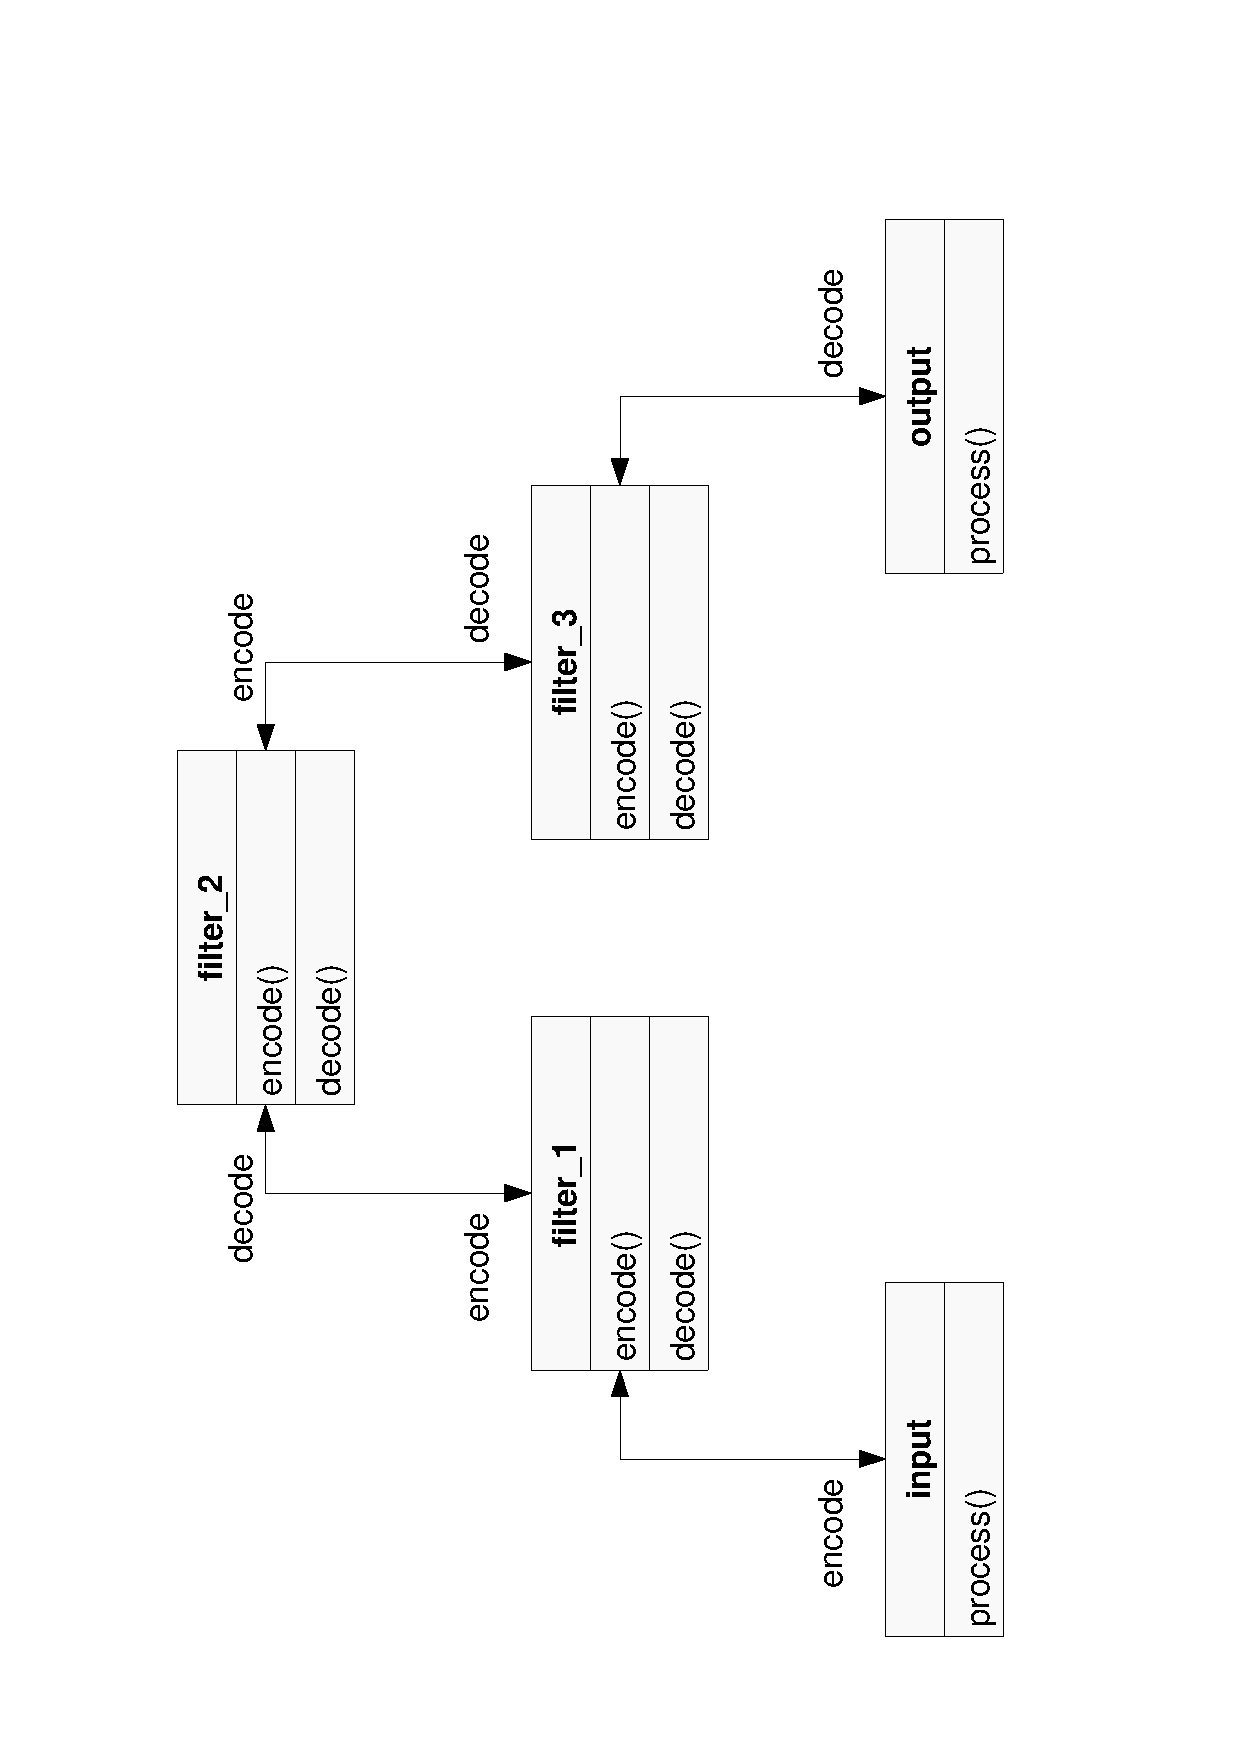
\includegraphics[scale=0.3,angle=-90]{graphic/pipesfilters.pdf}
        \caption{Pipes and Filters Pattern}
        \label{pipesfilters_figure}
    \end{center}
\end{figure}

\begin{itemize}
    \item[-] \emph{Push:} active filter pushes data to passive filter
    \item[-] \emph{Pull:} active filter pulls data from passive filter
    \item[-] \emph{Mixed Push-Pull-Pipeline:} all filters may push or pull data
    \item[-] \emph{Independent Loops:} all filters are active and access pipeline data
\end{itemize}

Families of related systems can be formed by changing the single filter
positions. Special communication filters are also used in the interpreter
program of chapter \ref{cybernetics_oriented_interpreter_heading}. Its filters
belong to neither of the above-listed forms of data forwarding, because they
are all passive, controlled from an outside entity which is not a filter
itself.
